
\section{General Architecture}
\label{sec:architecture}


The goal of the re-developed HOPS architecture is provide a component-based design which allows for a greater degree of flexibility
in the types of operations that may be applied to VLBI data during fringe fitting, and avoid the semi-monolithic approach used in the past.
To do this, the software package to be delivered will primarily comprise of a set of loosely coupled libraries which can be composed
into an variety of calibration and fringe-fitting applications. Moreover, rather than attempting to identify and categorize all manner of data
types and data manipulation which may be required by future observations at the outset, a primary goal of this project is to provide a
relatively flexible set of data containers and operators along with a python plugin interface so as to allow for future extensions with minimal revision to the existing code.

For the foreseeable future, the main source of input data to this software will be provided by the DiFX correlator. However, this may not always
be the case, so in order to decouple the correlator from the post-processing software a conversion utility must be provided. This follows
the same paradigm as the current code, where a separate application (difx2mark4, which depends on the DIFXIO library) handles the conversion. However,
in this iteration we propose that this conversion utility operate mainly as a transparent pass-through, merely
converting the correlator output into the native post-processing data format, rather than applying any initial calibration/normalization (e.g. auto-corrs) or
other corrections to the data.

Once the data has been converted to the native post-processing format additional manipulation within the fringe-fitter will take place in several stages, such as normalization, data-flagging, a priori phase/delay and band-pass calibration, and finally fringe search. At intervening stages
both the data objects and data operator objects will be exposed to a python interface and hooks will be provided for external user scripts to 
access and directly modify the data and/or data operators. A extremely simplified diagram of the control flow of such a single-baseline fringe-fitter executable is shown in \ref{fig:fringe-fitter}. A multi-baseline global fringe-fitting algorithm will also be made possible by refactoring the HOPS code, however, the exact nature of this algorithm (e.g. Cotton-Schwab or baseline stacking, etc.) and whether it will best be implemented as a configurable option of a single fringe-fitting executable or as its own separate executable needs to be determine.

Upon completion of fringe fitting, the calibrated data with fringe solution applied will then be saved in a native binary format with the option to convert to an archival format (e.g. HDF5) via a simple conversion utility. Intermediate stages (with partial data corrections applied) may also optionally saved to the native format. It is also desired that
the export of a data flagging table and band-pass correction table be made possible, such an export tool may initially be implemented via user python script. If a multi-package (HOPS/AIPS/CASA) exchange format is adopted/specified then this feature could be made a built-in option in the refactored code.

In addition to the fringe fitter itself, a number of other post-fringing data analysis tools will also be provided. Most importantly are
a fringe plot utility for diagnostic information about the quality of an individual fringe, as well as the equivalent executables to \textit{alist} and \textit{aedit}, which summarize multiple fringe solutions and display condensed information about multiple scans respectively.
We intended to preserved the existing functionality of these executables, but expect to make the fringe-plot more flexible by providing options
to enable/disable various plotting items.


\begin{figure}[H]
\begin{center}
  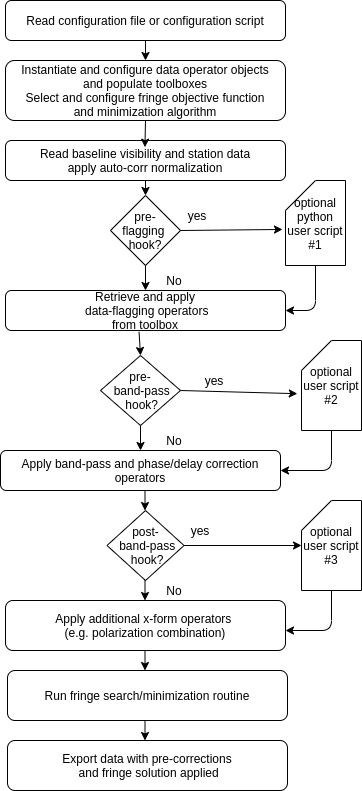
\includegraphics[width=0.6\textwidth]{fig/example-single-baseline-fringe-fitter.png}
    \caption{Example of simplified control flow for a single-baseline fringe fitter.}
    \label{fig:fringe-fitter}
\end{center}
\end{figure}
